\subsection {Выборочные коэффициенты корреляции}
	\begin{table}[H]
		\label{tabular:timesandtenses}
		\begin{center}
			\begin{tabular}{| c | c | c | c |} \hline 
 p = 0 & $r$ & $r_{S}$ & $r_{Q}$ \\ \hline 
 $E(z)$ & -0.009 & -0.007 & 0.002 \\ \hline 
 $E(z^2)$ & 0.051 & 0.053 & 0.054 \\ \hline 
 $D(z)$ & 0.051 & 0.053 & 0.054 \\ \hline 
 p = 0.5 & $r$ & $r_{S}$ & $r_{Q}$ \\ \hline 
 $E(z)$ & 0.486 & 0.456 & 0.326 \\ \hline 
 $E(z^2)$ & 0.269 & 0.243 & 0.154 \\ \hline 
 $D(z)$ & 0.032 & 0.036 & 0.048 \\ \hline 
 p = 0.9 & $r$ & $r_{S}$ & $r_{Q}$ \\ \hline 
 $E(z)$ & 0.895 & 0.867 & 0.694 \\ \hline 
 $E(z^2)$ & 0.803 & 0.756 & 0.509 \\ \hline 
 $D(z)$ & 0.002 & 0.005 & 0.027 \\ \hline 
 \end{tabular} 

		\end{center}
		\caption{Двумерное нормальное распределение, $n=20$}
	\end{table}

	\begin{table}[H]
		\label{tabular:timesandtenses}
		\begin{center}
			\begin{tabular}{| c | c | c | c |} \hline 
 p = 0 & $r$ & $r_{S}$ & $r_{Q}$ \\ \hline 
 $E(z)$ & 0.0 & 0.0 & 0.001 \\ \hline 
 $E(z^2)$ & 0.016 & 0.016 & 0.017 \\ \hline 
 $D(z)$ & 0.016 & 0.016 & 0.017 \\ \hline 
 p = 0.5 & $r$ & $r_{S}$ & $r_{Q}$ \\ \hline 
 $E(z)$ & 0.496 & 0.475 & 0.331 \\ \hline 
 $E(z^2)$ & 0.255 & 0.236 & 0.124 \\ \hline 
 $D(z)$ & 0.009 & 0.01 & 0.014 \\ \hline 
 p = 0.9 & $r$ & $r_{S}$ & $r_{Q}$ \\ \hline 
 $E(z)$ & 0.898 & 0.882 & 0.704 \\ \hline 
 $E(z^2)$ & 0.807 & 0.779 & 0.505 \\ \hline 
 $D(z)$ & 0.001 & 0.001 & 0.009 \\ \hline 
 \end{tabular} 

		\end{center}
		\caption{Двумерное нормальное распределение, $n=60$}
	\end{table}

	\begin{table}[H]
		\label{tabular:timesandtenses}
		\begin{center}
			\begin{tabular}{| c | c | c | c |} \hline 
 p = 0 & $r$ & $r_{S}$ & $r_{Q}$ \\ \hline 
 $E(z)$ & -0.003 & -0.002 & 0.002 \\ \hline 
 $E(z^2)$ & 0.01 & 0.01 & 0.01 \\ \hline 
 $D(z)$ & 0.01 & 0.01 & 0.01 \\ \hline 
 p = 0.5 & $r$ & $r_{S}$ & $r_{Q}$ \\ \hline 
 $E(z)$ & 0.494 & 0.474 & 0.328 \\ \hline 
 $E(z^2)$ & 0.25 & 0.231 & 0.117 \\ \hline 
 $D(z)$ & 0.006 & 0.006 & 0.009 \\ \hline 
 p = 0.9 & $r$ & $r_{S}$ & $r_{Q}$ \\ \hline 
 $E(z)$ & 0.898 & 0.885 & 0.706 \\ \hline 
 $E(z^2)$ & 0.807 & 0.784 & 0.503 \\ \hline 
 $D(z)$ & 0.0 & 0.001 & 0.005 \\ \hline 
 \end{tabular} 

		\end{center}
		\caption{Двумерное нормальное распределение, $n=100$}
	\end{table}

	\begin{table}[H]
		\label{tabular:timesandtenses}
		\begin{center}
			\begin{tabular}{| c | c | c | c |} \hline 
 n = 20 & $r$ & $r_{S}$ & $r_{Q}$ \\ \hline 
 $E(z)$ & 0.874 & 0.843 & 0.659 \\ \hline 
 $E(z^2)$ & 0.767 & 0.717 & 0.464 \\ \hline 
 $D(z)$ & 0.003 & 0.006 & 0.03 \\ \hline 


			
 n = 60 & $r$ & $r_{S}$ & $r_{Q}$ \\ \hline 
 $E(z)$ & 0.876 & 0.858 & 0.675 \\ \hline 
 $E(z^2)$ & 0.768 & 0.738 & 0.466 \\ \hline 
 $D(z)$ & 0.001 & 0.002 & 0.01 \\ \hline 


			
 n = 100 & $r$ & $r_{S}$ & $r_{Q}$ \\ \hline 
 $E(z)$ & 0.877 & 0.862 & 0.676 \\ \hline 
 $E(z^2)$ & 0.769 & 0.744 & 0.463 \\ \hline 
 $D(z)$ & 0.001 & 0.001 & 0.006 \\ \hline 
 \end{tabular} 

		\end{center}
		\caption{Смесь нормальных распределений}
	\end{table}

\subsection {Эллипсы рассеивания}
	\begin{figure}[H]
		\center{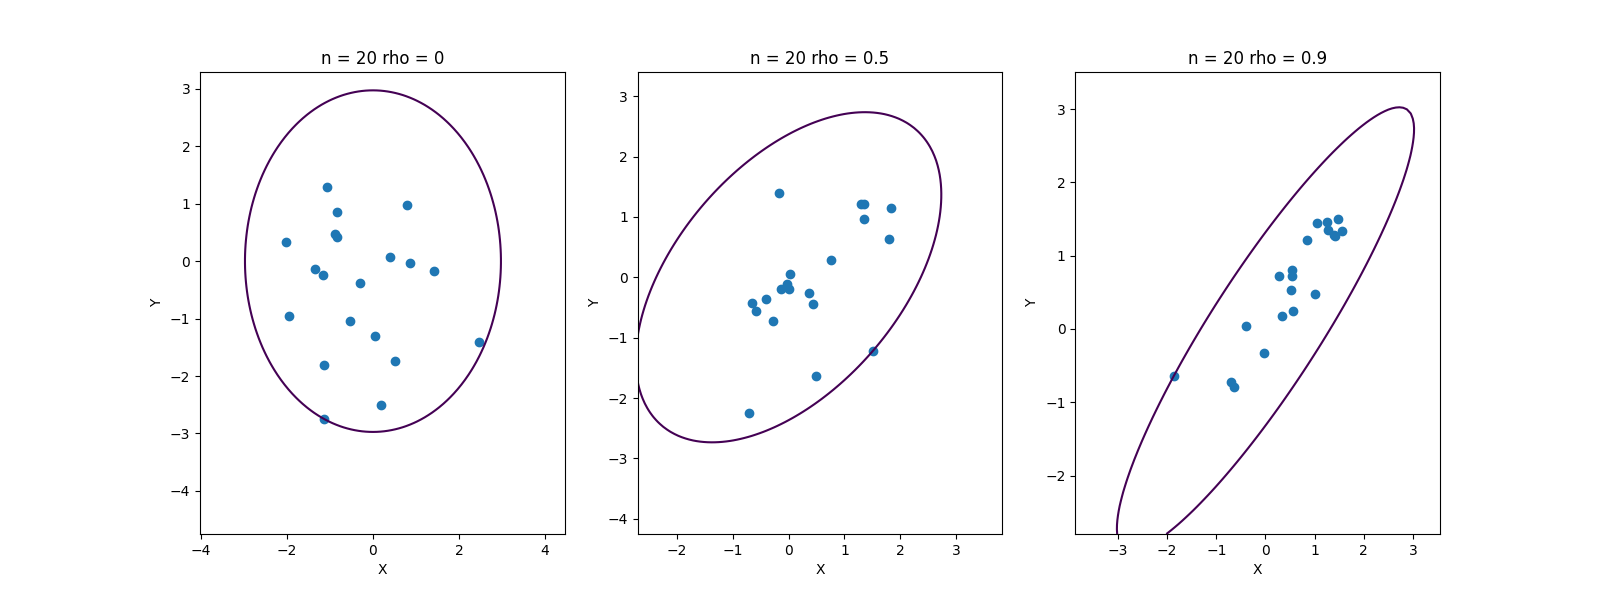
\includegraphics[width=1\linewidth]{20ellipse.png}}
		\caption{Двумерное нормальное распределение, n=20}
		\label{ris:image}
	\end{figure}

	\begin{figure}[H]
		\center{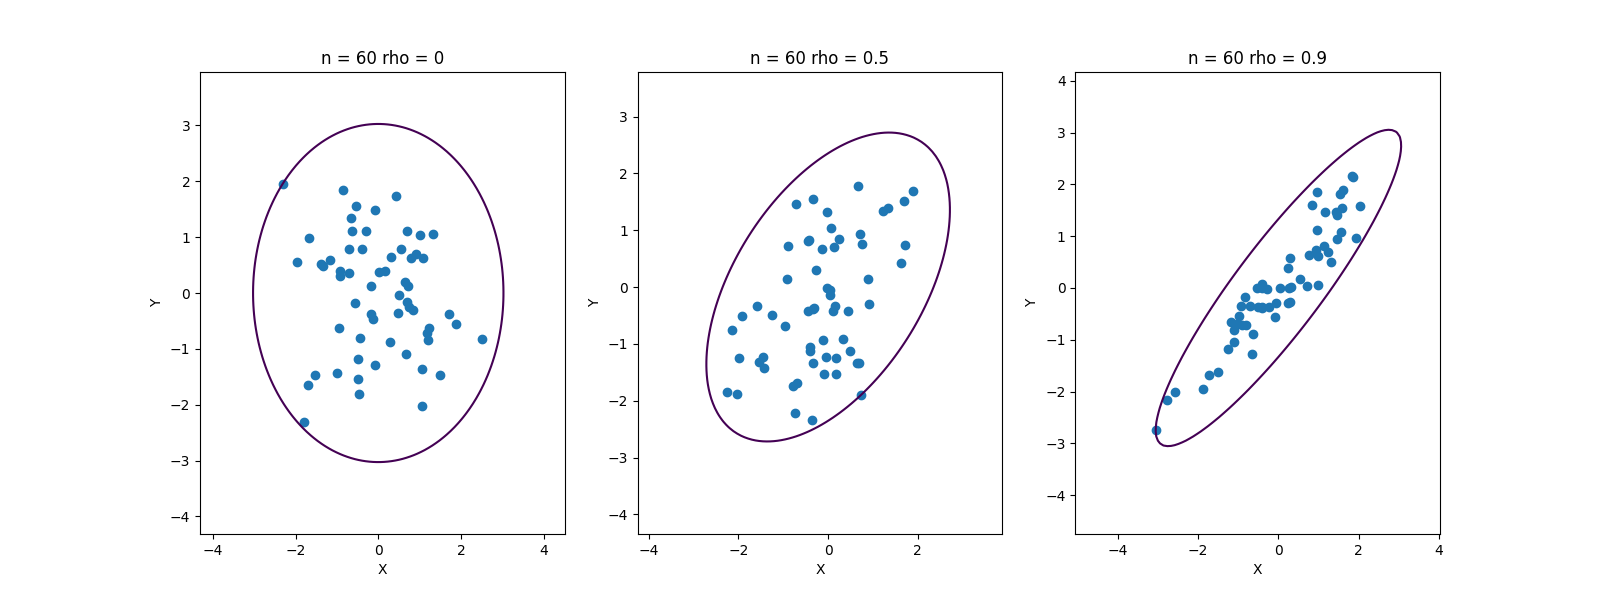
\includegraphics[width=1\linewidth]{60ellipse.png}}
		\caption{Двумерное нормальное распределение, n=60}
		\label{ris:image}
	\end{figure}

	\begin{figure}[H]
		\center{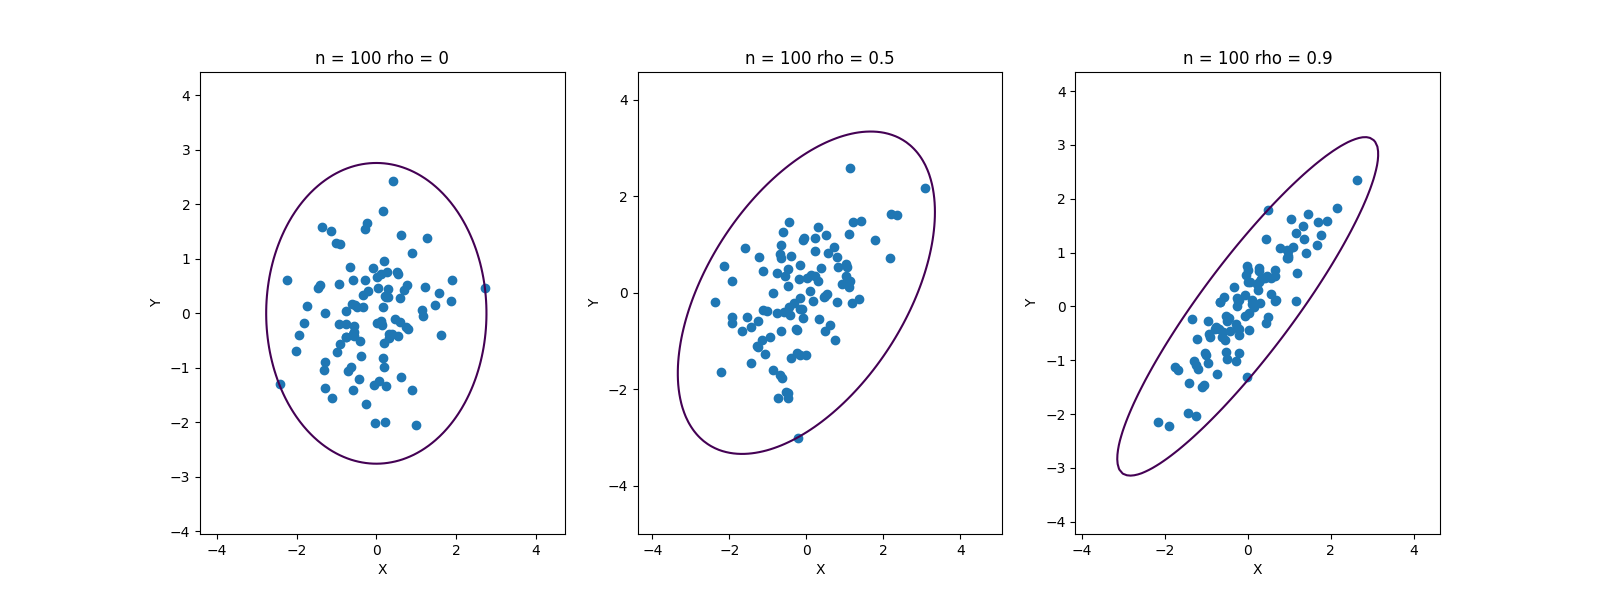
\includegraphics[width=1\linewidth]{100ellipse.png}}
		\caption{Двумерное нормальное распределение, n=100}
		\label{ris:image}
	\end{figure}

\subsection {Оценки коэффициентов линейной регрессии}
	\subsubsection {Выборка без возмущений}
		\begin{itemize}
			\item {Критерий наимеших квадратов:\\ $$\hat a \approx 1.868, \; \hat b \approx 1.738$$} 
			\item {Критерий наименьших модулей:\\ $$\hat a \approx 2.311, \; \hat b \approx 1.614$$}
		\end{itemize}

		\begin{figure}[H]
			\center{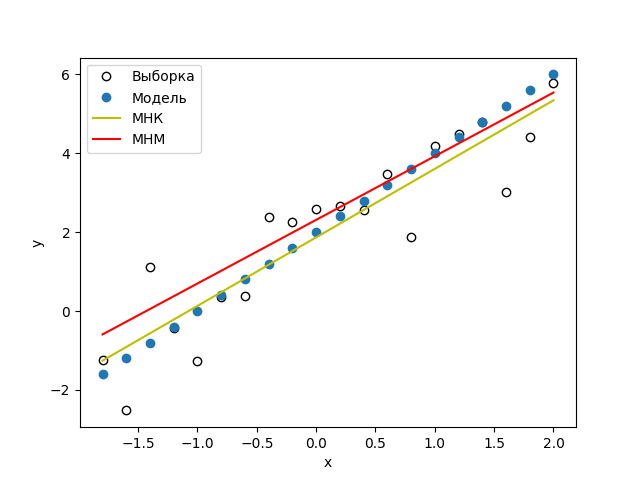
\includegraphics[width=0.5\linewidth]{default.png}}
			\caption{Выборка без возмущений}
			\label{ris:image}
		\end{figure}
	
	\subsubsection{Выборка с возмущениями}
		\begin{itemize}
			\item {Критерий наимеших квадратов:\\ $$\hat a \approx 1.786, \; \hat b \approx 0.052$$} 
			\item {Критерий наименьших модулей:\\ $$\hat a \approx 1.346, \; \hat b \approx 1.445$$}
		\end{itemize}

		\begin{figure}[H]
			\center{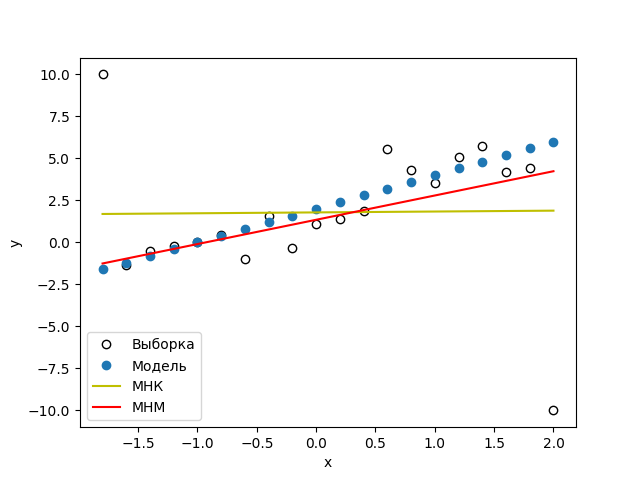
\includegraphics[width=0.5\linewidth]{default_with_distrubance.png}}
			\caption{Выборка с возмущениями}
			\label{ris:image}
		\end{figure}

\subsection{Проверка гипотезы о законе распределения генеральной совокупности. Метод хи-квадрат}
	\begin{table}[H]
\label{tabular:timesandtenses}
\begin{center}
$\hat{\mu} \approx 0.044$, $\hat{\sigma} \approx 0.975$\\ 
\begin{itemize}
 \item {Количество промежутков $k=8$}
 \item {Уровень значимости $\alpha=0.05$}
 \item {$\chi^2_{0.95}=14.067$}
\end{itemize}
\begin{tabular}{| c | c | c | c | c | c | c |} \hline 
 i & Границы & $n_i$ & $p_i$ & $np_i$ & $n_i-np_i$ & $\frac{(n_i-np_i)^2}{np_i}$ \\ \hline 
1 & [-inf, -1.0] & 14 & 0.159 & 15.866 & -1.866 & 0.219\\ \hline 
2 & [-1.0, -0.667] & 10 & 0.094 & 9.384 & 0.616 & 0.04\\ \hline 
3 & [-0.667, -0.333] & 17 & 0.117 & 11.695 & 5.305 & 2.407\\ \hline 
4 & [-0.333, 0.0] & 10 & 0.131 & 13.056 & -3.056 & 0.715\\ \hline 
5 & [0.0, 0.333] & 12 & 0.131 & 13.056 & -1.056 & 0.085\\ \hline 
6 & [0.333, 0.667] & 13 & 0.117 & 11.695 & 1.305 & 0.146\\ \hline 
7 & [0.667, 1.0] & 6 & 0.094 & 9.384 & -3.384 & 1.22\\ \hline 
8 & [1.0, inf] & 18 & 0.159 & 15.866 & 2.134 & 0.287\\ \hline 
$\sum$ & - & 100.0 & 1.0 & 100.0 & 0.0 & 5.12\\ \hline 
 \end{tabular} 
\end{center}

	\caption{Вычисление $\chi^2_B$ при проверке гипотезы $H_0$ о нормальном законе $N(x, \hat\mu, \hat\sigma)$}
	\end{table}
	Исследование на чувствительность:\\
	Рассмотрим гипотезу $H_0^*$, что выборка распределена согласно закону $Laplace(x, \hat\mu, \frac{\hat\sigma}{\sqrt{2}})$\\
	\begin{table}[H]
\label{tabular:timesandtenses}
\begin{center}
$\hat{\mu} \approx 0.077$, $\hat{\sigma} \approx 2.029$\\ 
\begin{itemize}
 \item {Количество промежутков $k=5$}
 \item {Уровень значимости $\alpha=0.05$}
 \item {$\chi^2_0.95=9.488$}
\end{itemize}
\begin{tabular}{| c | c | c | c | c | c | c |} \hline 
 i & Границы & $n_i$ & $p_i$ & $np_i$ & $n_i-np_i$ & $\frac{(n_i-np_i)^2}{np_i}$ \\ \hline 
1 & [-inf, -1.0] & 4 & 0.159 & 3.173 & 0.827 & 0.215\\ \hline 
2 & [-1.0, -0.333] & 2 & 0.211 & 4.216 & -2.216 & 1.165\\ \hline 
3 & [-0.333, 0.333] & 7 & 0.261 & 5.222 & 1.778 & 0.605\\ \hline 
4 & [0.333, 1.0] & 3 & 0.211 & 4.216 & -1.216 & 0.351\\ \hline 
5 & [1.0, inf] & 4 & 0.159 & 3.173 & 0.827 & 0.215\\ \hline 
$\sum$ & - & 20.0 & 1.0 & 20.0 & 0.0 & 2.551\\ \hline 
 \end{tabular} 
\end{center}

	\caption{Вычисление $\chi^2_B$ при проверке гипотезы $H_0^*$ о $Laplace(x, \hat\mu, \frac{\hat\sigma}{\sqrt{2}})$}
	\end{table}
	Видим, что $\chi^2_B<\chi^2_{0.95}$, следовательно гипотеза о нормальности принимается.\\
	Рассмотрим гипотезу $H_0^*$, что выборка распределена согласно равномерному распределению$(x, \hat\mu, \sigma)$\\
	\begin{table}[H]
\label{tabular:timesandtenses}
\begin{center}
$\hat{\mu} \approx -0.222$, $\hat{\sigma} \approx 0.969$\\ 
\begin{itemize}
 \item {Количество промежутков $k=5$}
 \item {Уровень значимости $\alpha=0.05$}
 \item {$\chi^2_{0.95}=9.488$}
\end{itemize}
\begin{tabular}{| c | c | c | c | c | c | c |} \hline 
 i & Границы & $n_i$ & $p_i$ & $np_i$ & $n_i-np_i$ & $\frac{(n_i-np_i)^2}{np_i}$ \\ \hline 
1 & [-inf, -1.0] & 6 & 0.159 & 3.173 & 2.827 & 2.518\\ \hline 
2 & [-1.0, -0.333] & 5 & 0.211 & 4.216 & 0.784 & 0.146\\ \hline 
3 & [-0.333, 0.333] & 2 & 0.261 & 5.222 & -3.222 & 1.988\\ \hline 
4 & [0.333, 1.0] & 4 & 0.211 & 4.216 & -0.216 & 0.011\\ \hline 
5 & [1.0, inf] & 3 & 0.159 & 3.173 & -0.173 & 0.009\\ \hline 
$\sum$ & - & 20.0 & 1.0 & 20.0 & 0.0 & 4.673\\ \hline 
 \end{tabular} 
\end{center}

	\caption{Вычисление $\chi^2_B$ при проверке гипотезы $H_0^*$ о равномерном распределении}
	\end{table}
	Видим, что $\chi^2_B<\chi^2_{0.95}$, следовательно гипотеза о нормальности принимается.

\subsection {Доверительные интервалы для параметров нормального распределения}
	\begin{table}[H]
		\label{tabular:timesandtenses}
		\begin{center}
			\begin{tabular}{| c | c | c |} \\ \hline 
n = 20 & $m$ & $\sigma$ \\ \hline 
 & $-0.334 < m < 0.412$ & $0.606 < \sigma < 1.163$ \\ \hline 
 & & \\ \hline 
n = 100 & $m$ & $\sigma$ \\ \hline 
 & $-0.089 < m < 0.308$ & $0.88 < \sigma < 1.164$ \\ \hline 
 & & \\ \hline 
 \end{tabular} 

		\end{center}
		\caption{Доверительные интервалы для параметров нормального распределения}
	\end{table}

\subsection {Доверительные интервалы для параметров произвольного распределения. Асимптотический подход}
	\begin{table}[H]
		\label{tabular:timesandtenses}
		\begin{center}
			\begin{tabular}{| c | c | c |} \\ \hline 
n = 20 & $m$ & $\sigma$ \\ \hline 
 & $-0.301 < m < 0.379$ & $0.557 < \sigma < 3.282$ \\ \hline 
 & & \\ \hline 
n = 100 & $m$ & $\sigma$ \\ \hline 
 & $-0.086 < m < 0.305$ & $0.832 < \sigma < 1.327$ \\ \hline 
 & & \\ \hline 
 \end{tabular} 

		\end{center}
		\caption{Доверительные интервалы для параметров произвольного распределения. Асимптотический подход}
	\end{table}